\newpage
\setcounter{page}{9}
\setlength{\columnsep}{50pt}
\begin{multicols}{2}
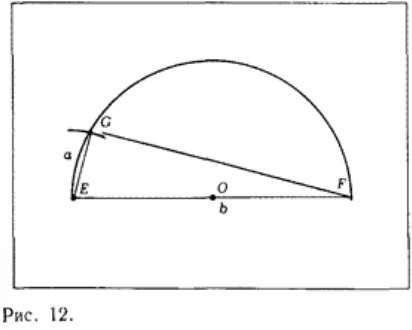
\includegraphics[scale=0.45]{ris_12.jpg}\par
№ 14. \textit{Построение} $\sqrt{b^2-a^2}$.\par
Разделим отрезок \textit{b - EF} пополам (см. № 7). Из центра \textit{O} проведем окружность $O_b$ радиуса \textit{b/2} (рис. 12). Из точки \textit{E} проведём засечку радиуса \textit{a}, пересекающую $O_b$ в некоторой точке \textit{G}. Отрезок \textit{FG} будет иметь нужную длину. Действительно, угол \textit{EGF} прямой, так как опирается на диаметр. Поэтому $(GF)^2=b^2-a^2$.\par
№ 15. Для построения отрезка $a\sqrt{3}$ напишем
  $$a\sqrt{3}-\sqrt{(2a)^2-a^2}$$
С помощью № 1 построим отрезок \textit{b = 2a} и применим № 14 к отрезкам \textit{b-2a} и \textit{a}.\par
№ 16. Запишем тождество
   $$a\sqrt{2}=\sqrt{(a\sqrt{3})^2-a^2}$$
Мы умеем строить $a\sqrt{3}$ и, значит, умеем строить $a\sqrt{2}$, применив № 14 к $b-a\sqrt{3}$ и \textit{a}.\par
№ 17. Запишем тождество
$$\sqrt{b^2+a^2}=\sqrt{(b\sqrt{2})^2-(\sqrt{b^2-a^2})^2}$$\par
Мы умеем строить $b\sqrt{2}$(см. №16) и $\sqrt{b^2-a^2}$ (см. № 14). Значит, умеем строить и $\sqrt{b^2+a^2}$.\par
Теперь мы можем решить нужную задачу.\par
Задача № 18. Найти пересечение окружности с прямой, проходящей через ее центр.\par
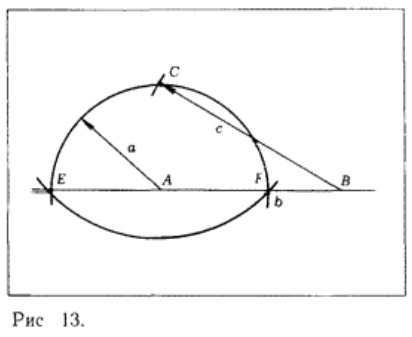
\includegraphics[scale=0.55]{ris_13.jpg}\newline
Решение. Пусть дана окружность $O_A$ с центром \textit{A} и точка \textit{B} $\neq$ \textit{A}. Нужно найти пересечение $O_A$ с прямой \textit{AB}. Обозначим радиус $O_A$ через \textit{a}, длину \textit{AB} через \textit{b} и построим \textit{с} $\sqrt{a^2+b^2}$ и $a\sqrt{2}$(см. № 16 и 17).\par
Теперь (рис. 13) из центра \textit{B} проведем засечку радиуса \textit{c} до пересечения с $O_A$ в некоторой точке \textit{C}. Из точки \textit{C} проведём окружность $O_C$ радиуса $a\sqrt{2}$. Пересечения $O_C$ и $O_A$ дадут искомые \textit{E} и \textit{F}.\par
Действительно, $\Delta$ \textit{BAC}-прямоугольный, ибо $c^2=a^2+b^2$. Если \textit{E} и \textit{F}-точки пересечения прямой \textit{AB} с окружностью $O_A$, то $(CE)^2=(CF)^2-2a^2$, как и было сделано.\par
Теорема Маскерони доказана полностью.\par
\par
\textbf{\S7. Зачем нужны построения циркулем без линейки}\newline
Хорошо известно, что математика не исчерпывается решением готовых задач, что она включает поиск проблем и постановку задач, формулировку теорем. Эта часть математики остается скрытой, хоть мы и знаем, что направляет работу именно она. А на проблеме построения циркулем хорошо видны задачи и решения именно <<второй>> части математики.\par
Когда мы смотрим кино, то видим актеров, а о том, что есть режиссер, только догадываемся. Должен ли режиссер оставаться за кадром? Мы решили однажды вывести его на сцену.

\end{multicols}

\newpage
\setcounter{page}{62}
\begin{minipage}{0.55\textwidth}
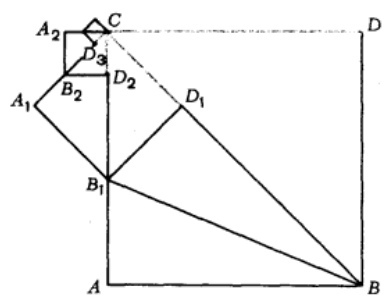
\includegraphics[scale=0.45]{ris_tab.jpg}\newline
нем отрезок $CA_1=D_1B_1$ и соединим точку $A_1$ с точкой $B_1$. Четырехугольник $A_1B_1D_1C$ - квадрат с диагональю $B_1C$.\par
Процесс построения квадратов можно продолжить. При этом мы получим бесконечную последовательность отрезков\newline
$ CD_1>CD_2>CD_3>CD_4>...>0;$
каждый из них есть разность между диагональю и стороной одного и того же квадрата; легко найти выражения для их длин:\newline
$CD_1=CB-AB,CD_2=CB_1-A_1B_1,...$
\end{minipage}
\hfill
\begin{minipage}{0.35\textwidth}
  \textbf{\Large Домино-пасьянс}\newline
  \newline
  28 косточек домино уложены в прямоугольник 7x8. Границы косточек не изображены. Требуется восстановить их.\newline
  \newline
  \begin{tabular}{|c c c c c c c|}
  \hline
  3 & 2 & 6 & 5 & 1 & 2 & 0\\
  2 & 1 & 5 & 4 & 5 & 4 & 5\\
  0 & 0 & 1 & 3 & 6 & 4 & 6\\
  0 & 5 & 5 & 3 & 4 & 4 & 0\\
  5 & 3 & 0 & 0 & 2 & 5 & 6\\
  4 & 0 & 3 & 2 & 6 & 6 & 6\\
  2 & 4 & 6 & 4 & 1 & 3 & 3\\
  2 & 2 & 1 & 1 & 1 & 1 & 3\\
  \hline
  \end{tabular}\newline
  а) \newline
  \newline
  \begin{tabular}{|c c c c c c c|}
  \hline
  4 & 3 & 1 & 3 & 5 & 5 & 5\\
  3 & 0 & 6 & 1 & 5 & 0 & 4\\
  0 & 0 & 4 & 2 & 0 & 1 & 5\\
  5 & 3 & 2 & 2 & 1 & 6 & 2\\
  0 & 4 & 4 & 4 & 2 & 5 & 4\\
  1 & 6 & 5 & 6 & 4 & 1 & 1\\
  0 & 3 & 6 & 6 & 3 & 1 & 2\\
  0 & 3 & 6 & 6 & 3 & 2 & 2\\
  \hline
  \end{tabular}\newline
  б)
  \begin{flushright}
  \textit{Л. П. Мочалов}
\end{flushright}
\end{minipage}